\section{Experimental design and results}
\label{sec:experiments}
\subsection{Public tables and fixed classifiers}
We use both main datasets requested for the study, German Credit and ACS Income, plus Pima Diabetes to obtain a lower-dimensional exact control. German has 20 original features; Pima has 8; ACS Income has 10. We use California 2018 ACS person records through folktables' standard task definition~\citep{ding2021}, not the Adult benchmark. The different dimensions make explicit when a budget reaches complete enumeration. They are not a controlled experiment isolating dimension from dataset content.

Each dataset has a stratified 75/25 training/test split. ACS training is capped at 20,000; the test pool is retained. We train logistic regression (LR), random forest (RF), and histogram gradient boosting (HGB) with fixed hyperparameters and seed. Logistic regression uses training-standardized numeric features and one-hot categorical variables; trees use original numeric/category codes. The games always use original features as players. Imputation is learned on training data. Table~\ref{tab:data} gives exact sample counts and predictive scores, which contextualize the fitted models but are not explanation-quality measures. Appendix~\ref{app:setup} specifies preprocessing and hyperparameters.

\begin{table*}[t]
\centering\small
\begin{tabular}{lrrrrrr}
\toprule
Dataset & $n$ & Train & Test & $d$ & LR/RF/HGB AUC & LR/RF/HGB acc. \\
\midrule
German & 1,000 & 750 & 250 & 20 & 0.762/0.780/0.788 & 0.728/0.708/0.720 \\
Pima & 768 & 576 & 192 & 8 & 0.821/0.824/0.796 & 0.781/0.755/0.750 \\
ACS & 195,665 & 20,000 & 48,917 & 10 & 0.892/0.883/0.897 & 0.814/0.805/0.817 \\
\bottomrule
\end{tabular}
\caption{Datasets after task filtering, training/test sizes and fixed-model predictive performance. LR/RF/HGB entries follow that order. ACS is unweighted California 2018 ACSIncome; its capped training sample does not change the test size.}
\label{tab:data}
\end{table*}

The main background is a fixed uniform sample of 16 training records, shared across cases and models within a dataset. This small background keeps online explanation costs realistic and makes the target completely explicit; it is not asserted to represent the population adequately. Each dataset contributes 32 uniformly selected test cases, matched across fitted models. There are \GameCount{} exact main games, \MainRuns{} stochastic main explanations across two estimators, and \DefaultRuns{} extra default-regularized Kernel explanations. Independent background redraws produce another \BackgroundGameCount{} exact games on eight cases per smaller dataset.

\subsection{Numerical accuracy and displayed-feature accuracy}
\label{sec:primary}
Table~\ref{tab:main} reports joint success, the fraction of runs satisfying both $E\leq .01$ and exact top-three equality. Every interval bootstraps the 32 cases in its cell. Figure~\ref{fig:accuracy} separates the two requirements. Over the nine equally weighted fitted-model cells, Kernel SHAP's joint success is \KernelLowJoint{} at $2d$, \KernelMediumJoint{} at $8d$, \KernelLargeJoint{} at $32d$, and \KernelHighJoint{} at $128d$. These averages describe this benchmark and are not a probability of reliability on an arbitrary future dataset.

At $8d$, numerical success is \KernelMediumNumeric{}, while top-three success is \KernelMediumRank{}. The criteria answer different questions: numerical tolerance controls all coordinates in probability units; a top-three display asks a discrete membership question. Relaxing the numerical tolerance to $.02$ yields \KernelMediumLenient{} numerical success, and tightening it to $.005$ yields \KernelMediumStrict{}. A threshold must therefore accompany any claim that an explanation is accurate enough. Material-sign success at this budget is \KernelMediumSign{}; including tiny near-zero features in a sign metric would ask a substantially more sensitive question.

\begin{table*}[t]
\centering\small
\begin{tabular}{llrrrr}
\toprule
Data & Model & $2d$ & $8d$ & $32d$ & $128d$ \\
\midrule
German & LR & 9.8 [6.3, 13.4] & 90.7 [84.5, 95.9] & 96.6 [92.9, 99.5] & 97.9 [94.4, 100.0] \\
German & RF & 20.3 [15.3, 25.5] & 91.3 [85.7, 96.2] & 96.2 [92.4, 99.2] & 98.4 [96.0, 99.9] \\
German & HGB & 0.3 [0.0, 0.8] & 48.6 [37.6, 59.1] & 95.8 [91.6, 98.8] & 98.6 [95.9, 100.0] \\
Pima & LR & 29.8 [22.1, 38.2] & 88.8 [81.3, 95.1] & 100.0 [100.0, 100.0] & 100.0 [100.0, 100.0] \\
Pima & RF & 23.5 [18.2, 29.1] & 92.7 [87.4, 96.9] & 100.0 [100.0, 100.0] & 100.0 [100.0, 100.0] \\
Pima & HGB & 1.1 [0.5, 1.7] & 40.2 [30.4, 50.5] & 100.0 [100.0, 100.0] & 100.0 [100.0, 100.0] \\
ACS & LR & 11.2 [6.9, 15.8] & 74.2 [64.8, 83.1] & 98.3 [95.5, 100.0] & 100.0 [100.0, 100.0] \\
ACS & RF & 16.5 [12.1, 21.0] & 91.1 [85.9, 95.2] & 99.5 [98.9, 100.0] & 100.0 [100.0, 100.0] \\
ACS & HGB & 2.2 [1.1, 3.4] & 52.1 [39.5, 64.7] & 91.4 [86.1, 95.6] & 100.0 [100.0, 100.0] \\
\bottomrule
\end{tabular}
\caption{Unregularized Kernel SHAP joint success: numerical maximum error at most $.01$ \emph{and} exact top-three set. Percent, with 95\% case-bootstrap intervals. Caps refer to interior coalitions and are further capped at complete enumeration of active columns. Each cell uses 32 cases and 64 seeds per case.}
\label{tab:main}
\end{table*}

\begin{figure*}[t]
\centering
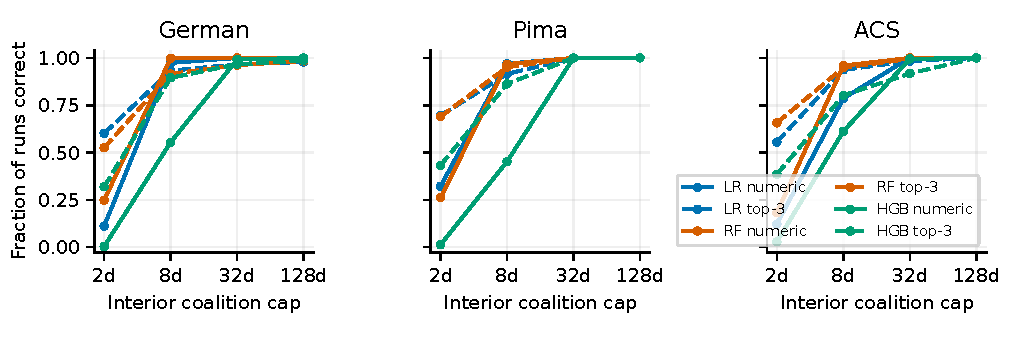
\includegraphics[width=\textwidth]{figures/accuracy.pdf}
\caption{Numerical success (solid) and exact top-three correctness (dashed), for the actual unregularized KernelExplainer. Lines are case-averaged descriptive means; joint-rate intervals appear in Table~\ref{tab:main}. Complete enumeration occurs by $32d$ for Pima and by $128d$ for ACS. The $128d$ German cap still samples only a small fraction of its coalition space.}
\label{fig:accuracy}
\end{figure*}

The smaller games reach an instructive positive control: Pima has only $2^8-2$ interior coalitions and ACS $2^{10}-2$. Their largest caps enumerate the whole active game, eliminating sampling randomness rather than merely reducing it. German's $128d$ cap remains approximate. Thus the high-budget overall mean should not be read as evidence that a fixed polynomial budget always suffices in higher dimensions. The nine cell means at $8d$ range from \CellMinMedium{} to \CellMaxMedium{}; the corresponding high-budget range is \CellMinHigh{} to \CellMaxHigh{}.

Averaging over inputs also hides difficult inputs. Pointwise lower-bound checks support $p_J\geq .95$ for \CertifiedMedium{} of 288 model/case pairs at $8d$ and \CertifiedHigh{} at $128d$. These checks require all 64 observed seeds to succeed; failing the check is inconclusive, not proof that $p_J<.95$. Passing cases at the exhaustive caps are deterministic controls for the chosen game. Neither their counts nor the bootstrap intervals certify every test input.

\subsection{Budget-matched permutation comparison}
\label{sec:baseline}
Figure~\ref{fig:baseline} compares joint success under the same interior-payoff caps. The reversal-paired permutation estimator is substantially stronger than low-budget Kernel SHAP in this experiment: its overall $2d$ joint success is \PermLowJoint{}, versus \KernelLowJoint{} for Kernel. At $8d$, it achieves \PermMediumJoint{}, and at $128d$, \PermHighJoint{}. This comparison neither establishes a universal winner nor implies that the same number of unique coalitions is spent: Kernel deduplicates while permutation paths can revisit a coalition and leave a remainder of the cap unused.

The lowest Kernel budget is close to the regression design's degrees of freedom, especially with complement pairing. The package emitted \WarningCount{} warnings in the main repetitions, retained together with all outputs; its singular-matrix fallback is not excluded. A warning-free run is also not a correctness certificate. At the largest smaller-game cap, Kernel's exact enumeration is a structural advantage over the random permutation baseline. The comparison identifies an interaction of budget and implementation, rather than a statement about the exact Shapley solution itself. A post hoc solver audit replays all \SolverRuns{} lowest-budget designs exactly: \ExtremePackage{} package outputs have $E>1$, versus \ExtremeSvd{} after replacing the normal-equation solve with SVD least squares. However, SVD only slightly improves low-budget success (Appendix~\ref{app:solver}); inadequate sampling remains a problem after extreme numerical failures are removed.

\begin{figure*}[t]
\centering
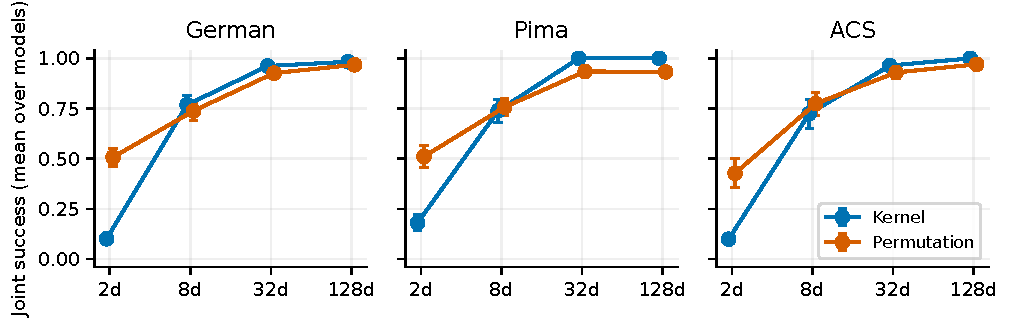
\includegraphics[width=\textwidth]{figures/baseline.pdf}
\caption{Joint success for Kernel SHAP and reversal-paired uniform permutation sampling under matched budget caps. Means average equally over the three fixed models. Error bars are 95\% bootstraps of matched cases within each dataset. Full enumeration benefits Kernel on the two smaller games; the permutation baseline continues random path sampling.}
\label{fig:baseline}
\end{figure*}

\subsection{Near ties and repeat agreement}
\label{sec:ties}
Figure~\ref{fig:margin} stratifies the $8d$ Kernel results by the exact third-versus-fourth absolute-attribution gap. The numerical and ranking criteria separate most clearly in the small-gap stratum. This descriptive analysis is consistent with Eq.~\eqref{eq:margin}; it does not identify the gap as the sole cause of error, because gap, model and data difficulty co-vary. There are \TiedCases{} exact or numerically negligible ($<10^{-12}$) cutoff ties among the 288 main model/case games. A deterministic tie rule makes the metric reproducible, not substantively important.

Two runs can choose the same incorrect set. Pooling disjoint seed pairs with equal dataset/model weights, the estimated fraction of agreeing top-three pairs that agree on a wrong set is \WrongAgreeLow{} at $2d$, \WrongAgreeMedium{} at $8d$, and \WrongAgreeHigh{} at $128d$. These are conditional descriptive rates with matched-case bootstrap uncertainty; they are not predictions for a deployment that selects its own examples or thresholds. Their purpose is to show why observing agreement and measuring target correctness are different operations. The released per-case analysis also measures agreement requiring numerical closeness.

\begin{figure}[t]
\centering
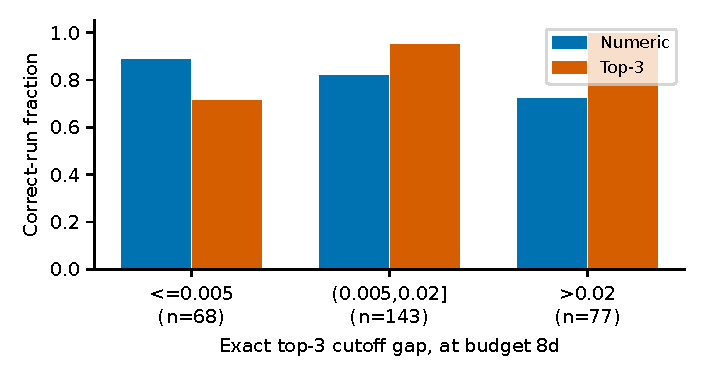
\includegraphics[width=\columnwidth]{figures/margin.pdf}
\caption{Descriptive $8d$ Kernel accuracy by exact top-three cutoff gap. Counts are model/case games, with the same test cases reused across models; bars are not independent-population estimates. Close rankings can change even when the numerical tolerance is met.}
\label{fig:margin}
\end{figure}

\subsection{Settings that change the answer}
\label{sec:ablations}
\paragraph{Default feature selection.}
Table~\ref{tab:reg} compares unregularized Kernel SHAP with its default top-10 feature selection on German Credit at $128d$, using the same coalition seeds. A sparse output is not the unrestricted target of Eq.~\eqref{eq:shap}. Consequently, increased repeatability does not automatically mean improved full-vector accuracy. For HGB, default repeat top-three agreement is \DefaultHGBRepeat{}, but numerical success is only \DefaultHGBNumeric{}. For LR, numerical success is \DefaultLRNumeric{}. The ablation reports both numerical and top-three accuracy alongside repeat top-three agreement; it should not be described as isolated Monte Carlo noise. All 20 original players remain in the reference even when the estimator selects only ten.

\begin{table*}[t]
\centering\small
\begin{tabular}{llrrr}
\toprule
Model & Regularization & Numeric & Top-3 & Repeat top-3 \\
\midrule
LR & None & 100.0 [100.0, 100.0] & 97.9 [94.4, 100.0] & 97.1 [92.8, 100.0] \\
LR & Top 10 & 0.0 [0.0, 0.0] & 78.3 [63.7, 90.6] & 91.7 [84.4, 97.6] \\
RF & None & 100.0 [100.0, 100.0] & 98.4 [96.0, 99.9] & 97.5 [94.2, 99.8] \\
RF & Top 10 & 92.4 [83.7, 99.3] & 93.7 [85.6, 99.1] & 95.3 [90.9, 98.9] \\
HGB & None & 100.0 [100.0, 100.0] & 98.6 [95.9, 100.0] & 98.4 [95.3, 100.0] \\
HGB & Top 10 & 12.4 [3.2, 23.0] & 93.6 [84.1, 100.0] & 98.5 [96.7, 100.0] \\
\bottomrule
\end{tabular}
\caption{German, $128d$: numerical correctness, top-three correctness and repeat top-three agreement. Percent with 95\% case-bootstrap intervals. ``Top 10'' is the actual SHAP 0.51.0 default, not an assumed default for other versions. Coalition seeds are paired with the unregularized condition.}
\label{tab:reg}
\end{table*}

\paragraph{Background redraws change the target.}
For Pima and ACS, we use eight selected inputs, all models, and eight independent training-background draws at each of $B=4,16,64$. We compute exact Shapley values under each draw, so disagreement here cannot be blamed on the attribution estimator. Table~\ref{tab:bg} compares all 28 pairs of backgrounds within each case, keeping those dependent pairs inside a case for inference. Increasing $B$ improves numerical agreement, but need not make a strict top-three display identical. These are comparisons between finite-sample targets, not errors relative to a known population-background Shapley value. The smaller sample of eight cases warrants cautious interpretation of its intervals.

\begin{table*}[t]
\centering\small
\begin{tabular}{llrrr}
\toprule
Dataset & $B$ & Top-3 agreement & $\|\Delta\phi\|_\infty\leq .01$ & Mean $\|\Delta\phi\|_\infty$ \\
\midrule
Pima & 4 & 34.7 [25.1, 44.2] & 0.0 [0.0, 0.0] & 0.104 [0.085, 0.125] \\
Pima & 16 & 54.6 [43.2, 66.5] & 0.3 [0.0, 0.7] & 0.067 [0.057, 0.077] \\
Pima & 64 & 82.3 [69.9, 93.8] & 7.3 [4.8, 10.4] & 0.027 [0.024, 0.031] \\
ACS & 4 & 17.3 [11.0, 24.3] & 0.0 [0.0, 0.0] & 0.132 [0.121, 0.144] \\
ACS & 16 & 30.7 [24.6, 37.6] & 0.0 [0.0, 0.0] & 0.064 [0.057, 0.072] \\
ACS & 64 & 56.1 [46.6, 66.2] & 2.8 [1.5, 4.2] & 0.030 [0.028, 0.032] \\
\bottomrule
\end{tabular}
\caption{Agreement of \emph{exact} explanations across independent background draws. Model means receive equal weight; intervals bootstrap the eight matched cases in each dataset, conditional on the eight saved draws per case/size. Top-three and numerical-agreement entries are percentages; maximum-error differences are in probability units.}
\label{tab:bg}
\end{table*}

\paragraph{Averaging and real cost.}
Four-run averaging of the lowest-budget package estimates is markedly worse than a single $8d$ run in all three datasets (Appendix~\ref{app:averaging}). This is a result for this low-budget implementation, partly affected by extreme numerical outputs; it is not a general argument against independent averaging. The comparison reports endpoint and saturation caveats rather than assuming perfect cost equality. Appendix~\ref{app:timing} reports direct, uncached online timings. Across the measured cells, median Kernel latency ranges from \TimeMin{} to \TimeMax{} milliseconds on the constrained CPU host. These use one input per cell and include contention; a production latency budget should be profiled on its own hardware and input distribution.
